\documentclass[12pt,a4paper]{report}
\usepackage[utf8]{inputenc}
\usepackage{csquotes}
\usepackage{graphicx}
\graphicspath{{Figures/}}
\usepackage[top=25mm,bottom=25mm]{geometry}
% to change text color.
\usepackage{xcolor}
% for url.
\usepackage{hyperref}
% to be able to comment out text.
\usepackage{verbatim}
% package for references:
\usepackage[style=alphabetic]{biblatex}
\addbibresource{references.bib}

\title{
    {\large Luleå University of Technology}\\
    {\large Department of Computer Science, Electrical and Space Engineering}\\
    {\large Digital Services and Systems}\\
    {\large COURSE: D0005N}\\
    {CASE STUDY: Census Bureaus}\\
    {\centering
\includegraphics{LTUlogo.png}}\\
}

\author{Anna Emmer-Granqvist, Kim Sandlund, Martin Tulestedt}
\date{March X 2025}

\begin{document}

\maketitle

\chapter*{Abstract}
This is the summary of the document ...


\chapter*{Highlights}
This is the assignment highlights on which we would like to highlight the following points that we think are key:
\begin{itemize}
    \item Theory 
    \item Practice
    \item Others
\end{itemize}

\tableofcontents

\chapter{Question One}
We suggest that the Business Intelligence (BI) -architecture for Census Bureaus should consist of several interconnected layers, 
in line with those outlined in the course literature \cite[chapter~31.2]{CourseLitt}, \cite{l2video}. 

The core BI-architecture includes four layers - a source data layer, an extract-transform-load (ETL) layer, 
a data warehouse (DW) layer and an end-user layer. 
The end-user layer is at the top of the BI- architecture, followed by the DW layer. 
The source data layer is at the bottom of the architecture, from perspective of end users. 
Our answer in this case question Q1 emphasizes the DW layer and the end-user layer, 
given that BI-technologies are typically defined as the combination of DW technologies and 
related analytical tools mainly for Online Analytical Processing (OLAP) and data mining \cite[chapter~33.]{CourseLitt}.  

\begin{figure}[h] % "h" means "here"
  \centering
  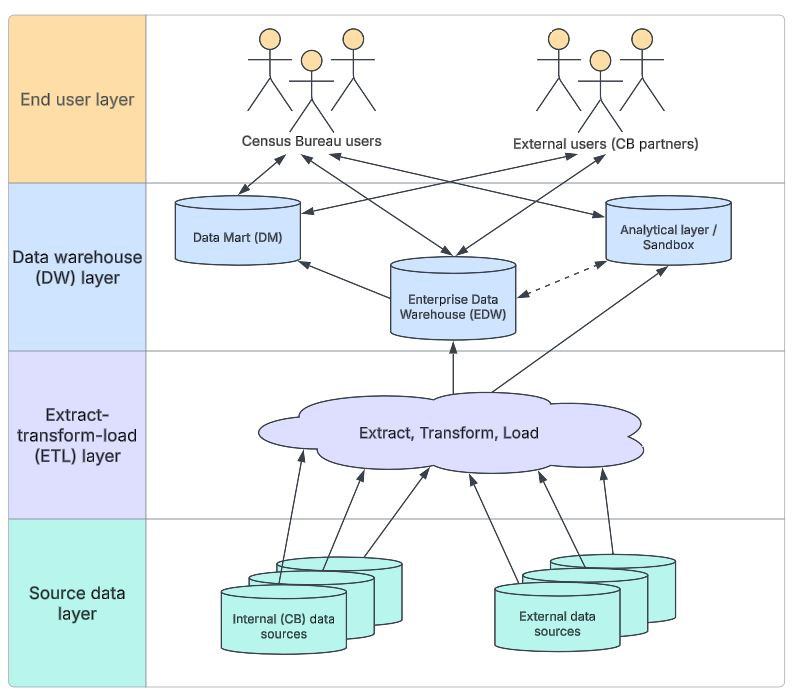
\includegraphics[width=1.0\textwidth]{Figures/Q1_BI_architecture.jpg}
  \caption{Proposed layered BI architecture for Census Bureaus.}
  \label{fig:BI_arch}
\end{figure}
\newpage
As regards the ETL-layer, it is a compulsory part and component of any DW/BI-architecture, 
also in this case of Census Bureaus. 
Same with the data source layer, it is required in any constellation of a DW/BI-architecture. 
But what is particular in this case is that we believe Census Bureaus by default have 
several external data sources. 
And that most of these are tied to other authorities, 
either national (subject-specific) or regional (location-specific). 
But as or when data from the various internal and external data sources have been successfully loaded into 
the data warehouse, the main interest is in the DW layer and the end-user layer.  

To Census Bureaus our group recommends a DW layer having an enterprise data warehouse (EDW) 
as its foundation, but which is supplemented by a limited number of Data marts (DM). 
Here the EDW can be defined as a common storage of all historical data collected and 
gathered by a Census Burau. 
It means that the EDW represents the combined data model for a given Census Burau as a whole, 
and for all of its subject areas \cite[chapter~32.2]{CourseLitt}. 
In in our BI-architecture the EDW provides all of the data to the data marts, 
whereas the data marts transfer no data to the EDW. 
These data marts could thus be categorized as dependent DM:s \cite{l2video}. 
The rationale for having an EDW as the main DW component is that it is the best alternative for 
gaining a consistent and 
all-encompassing view on the wide and diverse data held by a Census Bureau \cite[chapter~32.2]{CourseLitt}. 
As Census Bureaus are central nodes for census data and other statistics in their respective nations, 
it is important that they as national authorities can act as the “single source of the truth”. 
Having an EDW implemented enables this. 
Another strength of the EDW is that it is more flexible than data marts \cite{l3video}. 
This can be valuable for Census Bureaus e.g. if their data sources are volatile.  

The EDW that a given Census Bureau has should be accompanied by a limited number of separate data marts. 
The data marts should be allocated to the most important subject areas of that Census Bureaus. 
We think that the importance is partly dependent on the preferences of each Census Bureau, 
but generally those subject areas that are critical for society (healthcare, social insurance, energy) 
or that have large user groups (labour market, housing, construction) should be favoured. 
We think that the main advantage of implementing data marts for specific subject areas are 
that data can be supplied in forms that are tailored to the target user groups  \cite[chapter~31.4.1]{CourseLitt}. 
However, keeping the number of data marts moderate is crucial, as to avoid creating a duplicate DW layer 
that would accelerate costs while impairing overall DW performance.   

One important component that must be part of the DW layer is the warehouse manager. 
One of the main reasons for this is that warehouse managers are able to de-normalize data models and 
tables in the DW \cite[chapter~31.2.4]{CourseLitt}. 
This feature is essential, as it enables analytical tools such as OLAP and 
data mining to access the EDW directly. 
However, in the figure describing our layered BI-architecture, 
we interpret the warehouse manager as an integrated part of the EDW.  

Analytic platforms, also known as sandboxes, 
are another component that adhere to the DW layer \cite{l2video}. 
These solutions are implemented and operate separate from the EDW, 
whereby they offer users own environments for storing unstructured data and 
experimenting with that to discover new patterns. 
Given the unstructured nature of the data and the experimental potentials in a sandbox, 
security becomes an important factor. 
As such, we recommend that only certain personnel employed at the given Census Bureau (power users) 
is given access to it.  
The main usefulness of the sandbox is given by combining data sets from divergent subject areas, 
as to discover previously unknown associations or patterns. 
Another area of great use is to experiment with data before implementing it in the EDW 
to ensure compliance with the EDW and other factors. 
As such, the sandbox needs access to data beyond that of the EDW, 
which does not have as stringent, or necessarily any, demands on data transformation. 
In order to not overly complicate our architecture figure, 
we have however shown that it fetches data from the ETL layer like the EDW does. 
However, in practice the sandbox would have its own data fetch process. 
We recommend that Census Bureaus implement either physical sandboxes or 
software-as-a-service (SaaS) sandboxes \cite{l2video}. 
For more information about the usefulness of sandboxes for Census Bureaus, please see case question Q2.  

 

End user layers are in practice mandatory in BI-architectures of Census Bureaus. 
Without them users would be unable to analyse data in a DW, 
whereby the DW and all of its components would be more or less useless. 
The tools in the end user layer can be divided into four groups dependent on whether they are used for:\cite[chapter~31.2.10]{CourseLitt}
\begin{enumerate}[label=\roman*)]
  \item traditional queries and reports
  \item OLAP purposes
  \item data mining
  \item application development
\end{enumerate}

We argue that Census Bureaus need to invest in and take into active use tools belonging to the categories i-iii, 
as all three are necessary and as they complement each other. 
OLAP tools are needed for detailed and ad-hoc analyses of 
multidimensional data sets of larger sizes \cite[chapter~33.1]{CourseLitt}. 
Data mining tools, in turn, are optimal to apply on extensive data sets, 
also called big data \cite[chapter~34.1]{CourseLitt}.  
A final thing that our group includes in the end user layer is a visualisation tool. 
Most often tools of this type are either integrated into OLAP tools \cite{l4video}. 
But if not, then a Census Bureau should install a separate visualization tool as to 
have it part of its BI-architecture. 
Data visualization has become increasingly popular as data grow in volume and complexity. 
Here the potential user groups include external users of Census Bureaus as well as citizens.  

\chapter{Question Two}
Question:\\
\emph{
    What would be the role of sandboxes – in your opinion – in government decision-making?
}\\\\
\emph{[00:09:33] the second is the role of sandboxes i also explained the sandboxes do you think that the government decision making needs sandboxes
yeah then it's not only a binary question that you say yes or no too but you also have to give some insights
why you think they need or do not need a sandbox}\\\\
What to do here?
\begin{enumerate}
    \item research and discuss sandboxes
    \begin{enumerate}
    \item Find Lecture where he talks about sandboxes, take note of relevant slides.
    \footnote{Lecture name: Y, Slide: X}
    \item Summarize said lecture findings in document
    \item Include summary here or share in Discord under Resources.
    \end{enumerate}
    \item write about pros and cons of sandboxes in government decision-making
    \item summarize and write about the role of sandbozes in government decision-making
  \end{enumerate}

\newpage Answers to Question 2:(ANNA RESEARCH REFERENCES)

\newpage 
'text in single quotation'

''text in double quotations''\\

One of today’s key technologies is \textbf{Big Data}\\
One of today’s key technologies is \textit{Big Data}\\
One of today’s key technologies is \underline{Big Data}\\

Here I am referring to the source \cite{BigData}.

\chapter{Question Three}
Question:\\
\emph{
    How can the Census Bureau justify its investment in data warehousing and mining
technologies?
}\\\\

\emph{[00:09:56] then third is justify the investment do you think the investment that governments make worldwide
and and and they do actually um in data warehousing and data mining is justified is the return on investment
up in the case i explained some benefits but i also need you not only to take a copy of that but
to discuss it do you think yes it brings value back to them how do you think would that value be
identified and reaped and attained by those governments}\\\\
how do you think would that value be
identified and reaped and attained by those governments
data warehousing and data mining is justified is the return on investment

What to do here?
\begin{enumerate}
    \item motivate why data warehousing is a good idea for the Census Bureau
    \item motivate why data mining is a good idea for the Census Bureau
  \end{enumerate}

\newpage Answers to Question 3: (KIM RESEARCHES REFERENCES)
KIM DOES THIS IN WORD AND THEN PUTS IT HERE. ACCESIBLE VIA LINK:\\
\url{https://ltuse-my.sharepoint.com/:w:/g/personal/sankim-3_student_ltu_se/EVlVl5wzZJpJgSEYamfwzagBWiYV15YG1EIvPHk9yXiOBQ?e=fwckui}

There are several different types of advantages that organisations can gain by making investments in data warehousing (DW) and data mining technologies.
\\\\
Obtaining access to a data warehouse and to associated tools for analysing that data is very valuable for any Census Bureau, 
because it implies a shift from “multiple sources of truths“ to a “single source of truth” \cite{l2video}. 
By implementing DW together with tools, a Census Bureau can consolidate its multiple data sources representing different areas -- 
such as population, society and economy -- into one aggregated pool of data. 
This, in turn, gives a bureau more comprehensive views together with entirely new insights on the data it possesses. 
A bureau can thus discover new patterns in its data but, also falsify earlier believes it had about certain data. 
This is a very important issue, 
as it can be assumed that a typical challenge for Census Bureaus is that they and their customers struggle with multiple information silos, 
many of which are disintegrated rather than integrated.
\\\\
Data and information have become critical success factors for almost all organizations. 
And DW together with its tools supplies its users with entirely new and usually very valuable information \cite[chapter~31.1.3]{CourseLitt}. 
Consequently, one of the foremost arguments for a Census Bureau to opt for DW and data mining is that it can provide a competitive advantage \cite{l2video}. 
Not only for the bureau, but also for the government it serves and for other parties utilizing the information and services provided by the bureau. 
Considering that DW and data mining as technologies have become increasingly popular during the past one-two decades, 
it is perhaps more appropriate to state that these technologies are almost inevitable investments for any Census Bureau today. 
Without DW and analytical tools such as online analytical processing (OLAP) and data mining, 
a Census Bureau would not be able to serve its customers to the full. 
At the same time, it would have a competitive disadvantage towards its national and international peers.
\\\\
As data warehousing and analytical tools are expected to result in new information and a better understanding among the users,
it should eventually also lead to better decisions \cite[chapter~31.1.3]{CourseLitt}. 
This would be a particularly important consequence for an organization like a Census Bureau, 
which serves a broad group of stakeholders covering governments, 
various public and private organizations and also citizens. 
Making better decisions, based on more accurate information, would benefit all parties that utilize the DW and -tools of a Census Bureau. 
The positive effects could on an aggregate level, for the whole society, become substantial.
\\\\
An apparent gain that comes with DW and its tools is the flexibility they provide to those using them. 
Whereas traditional databases such as OLTP-systems are designed to handle fairly simple but high-volume data transactions, DW:s can handle many
different types of queries -- also those being very complex, detailed or multi-conditional \cite[chapter~31.1.4]{CourseLitt}. 
DW would thus be a valuable change for all parties acquiring data from Census Bureaus, 
as it would broaden the scope of queries that are possible for them. 
Moreover, acquiring data though these queries would for Census Bureau users also become easier and faster than before.
\\\\
The technologies of data warehouses have evolved steadily over the years, 
and one area where this applies is the time delays between data in operational sources and in DW:s \cite[chapter~31.1.6]{CourseLitt}. 
The time delays have been reduced and DW:s have evolved towards what can be called real-time (RT) or near real-time (NRT) data warehouses (Coursebook, 31.1.6; Lecture 2-20250213AE). 
This means that data in DW:s is nowadays more current than it was before, 
which in turn shortens the time cycles for making informed decisions. 
Making faster decisions enabled by modern DW technologies would be beneficial for a Census Bureau and its stakeholders, 
as faster decisions can provide decision makers with competitive advantages.
\\\\
One operational gain that can be obtained from DW and data mining is that the implementation process enables and often motivates organizations to
unify terms and definitions for different types of data \cite{l2video}. 
All data that is extracted, transferred and loaded into a DW needs to be harmonized so that it can be used for analyses. 
This would be beneficial for a Census Bureau, which typically obtains and manages data from multiple sources, 
but where uniform data can differ in terms or definitions. 
Unified terms and definitions for same data would improve the quality of the data itself and the Census Bureau operations overall.
Data warehousing could potentially enable a Census Bureau to combine and analyse multiple sets of data that it has not analysed before.
\\\\ 
Altogether it appears clear that investing in data warehousing and in tools such as OLAP or data mining can generate many positive yet 
different effects for a Census Bureau. 
The effects described and elaborated on above are primarily operational, as they relate to things such as more and better information,
and better and faster decision-making. 
If or when this is the case, it should also have financial implications for a Census Bureau and its customers.
On a general level, implementing DW and its tools have in the past been very profitable investments. 
These investments have showed return rates (ROI) of several hundred percent,
together with payback periods measured in months rather than years \cite[chapter~31.1.3]{CourseLitt}, \cite{l2video}. 
Although a Census Bureau itself is a non-profit organization, 
it is justified that it invests in DW technologies as to improve the profitability of its public and private customers. 
Although such investments would expand the budget of a Census Bureau in the short term, 
in the longer term it would most likely be counterweighted by higher tax revenues from society.

\chapter{Question Four}
\section{Logical design of a data warehouse for Census Bureaus}
We have designed a limited dimensional model that could be implemented by a Census Bureau. 
The model is classified as star schema as it has only fact table which is connected to a number 
of denormalized dimension tables \cite[chapter~32.4]{CourseLitt}. The theme chosen for this star schema was 
residence permits in Sweden, which constitutes a part of migration and which among Census Bureaus 
belongs to the subject area “Population”. Depending on the scope and perspective, residence permits 
potentially also connects to “Living conditions” and “Housing”. The motivation of us to design a DW 
about residence permits is mainly to obtain a statistical tool that creates insights about persons 
who have been granted residence permits in Sweden. As to first gain a better understanding of common 
features among the target group, and then to help local, regional and national decision makers in 
Sweden to improve the overall lives of persons with residence permits. 

The star schema that the group created consists of the fact table ResidencePermits, whose primary 
key is a composite key consisting of five foreign keys stemming from each dimension table. The fact 
table contains three fact attributes or facts, which are: permanentResPermits, temporaryResPermits and 
totalResPermits. As the table name and fact attributes suggest, they refer to the quantitative number 
of residence permits granted to individuals in a certain country, in this example in Sweden. Here the 
residence permits have been divided into two additive types, permanent and temporary. Also, total 
permits has been included, which is registered separately but which should equal the sum of the former two types. 

The fact table has been accompanied by five dimension tables. Each of these contains one surrogate 
type of primary key together with five attributes relating to the dimension in question. The measures 
of the attributes vary within and across dimension tables, but most of them are qualitative. All five 
dimensions Time, Domicile, Background, Socioeconomics and Living - including their attributes - have 
relationships with ResidencePermits as the fact being analysed. It is worth noting that the individual 
facts in the fact table are independent from all other attributes in the dimension tables, except for the 
two attributes residencePermitCat and residencePermitDate, which are implicitly interrelated with each of 
the three facts (permanentResPermits, temporaryResPermits and totalResPermits). 
\newpage
\subsection{Fact table and dimension tables (star schema)}
\begin{figure}[h] % "h" means "here"
  \centering
  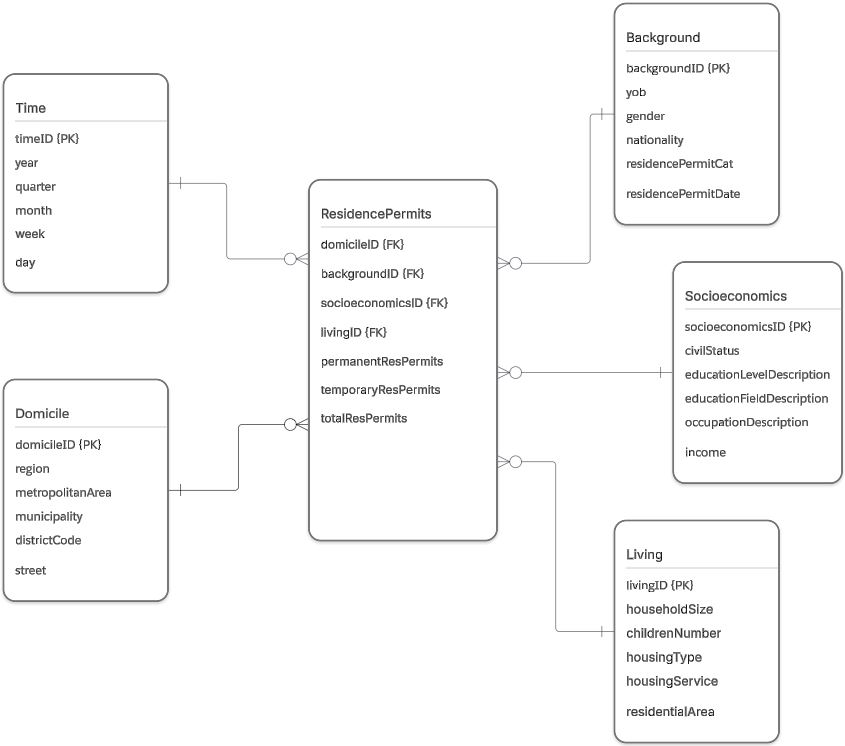
\includegraphics[width=1.0\textwidth]{Figures/Q4_StarSchema.jpg}
  \label{fig:my_image}
\end{figure}
\newpage
\subsection{Attribute descriptions for logical design}
% ResidencePermits (Fact table)
\begin{table}[htbp]
  \centering
  \caption{ResidencePermits (Fact table)}
  \begin{tabular}{|l|l|l|}
    \hline
    \textbf{Attribute} & \textbf{Domain} & \textbf{Data type} \\
    \hline
    timeID & Foreign Key & INT \\
    \hline
    foreignID & Foreign Key & INT \\
    \hline
    domicileID & Foreign Key & INT \\
    \hline
    backgroundID & Foreign Key & INT \\
    \hline
    socioeconomicsID & Foreign Key & INT \\
    \hline
    livingID & Foreign Key & INT \\
    \hline
    permanentResPermits & Number of granted permanent resident permits & INT \\
    \hline
    temporaryResPermits & Number of granted temporary resident permits & INT \\
    \hline
    totalResPermits & Total number of granted resident permits & INT \\
    \hline
  \end{tabular}
\end{table}

% Time (Dimension table)
\begin{table}[htbp]
  \centering
  \caption{Time (Dimension table)}
  \begin{tabular}{|l|l|l|}
    \hline
    \textbf{Attribute} & \textbf{Domain} & \textbf{Data type} \\
    \hline
    timeID & Primary Key, auto increment & INT \\
    \hline
    year & Year & INT \\
    \hline
    quarter & number of a quarter of a year & SMALLINT(1-4) \\
    \hline
    month & Month number & SMALLINT(1-12) \\
    \hline
    week & Week number & SMALLINT(1-53) \\
    \hline
    day & Day number & SMALLINT(1-31) \\
    \hline
  \end{tabular}
\end{table}

% Domicile (Dimension table)
\begin{table}[htbp]
  \centering
  \caption{Domicile (Dimension table)}
  \begin{tabular}{|l|l|l|}
    \hline
    \textbf{Attribute} & \textbf{Domain} & \textbf{Data type} \\
    \hline
    domicileID & Primary Key, auto increment & INT \\
    \hline
    region & Region name & VARCHAR \\
    \hline
    metropolitanArea & Metropolitan area name & VARCHAR \\
    \hline
    municipality & Municipality name & VARCHAR \\
    \hline
    districtCode & District code & VARCHAR \\
    \hline
    street & Street name & VARCHAR \\
    \hline
  \end{tabular}
\end{table}

% Background (Dimension table)
\begin{table}[htbp]
  \centering
  \caption{Background (Dimension table)}
  \begin{tabular}{|l|l|l|}
    \hline
    \textbf{Attribute} & \textbf{Domain} & \textbf{Data type} \\
    \hline
    backgroundID & Primary Key, auto increment & INT \\
    \hline
    yob & Year of birth & SMALLINT(4) \\
    \hline
    gender & Gender, M/F & CHAR(1) \\
    \hline
    nationality & Nationality & VARCHAR \\
    \hline
    residencePermitCat & Residence permit category (Work/EU-EES etc) & VARCHAR \\
    \hline
    residencePermitDate & Date of residence permit & DATE \\
    \hline
  \end{tabular}
\end{table}

% Socioeconomics (Dimension table)
\begin{table}[htbp]
  \centering
  \caption{Socioeconomics (Dimension table)}
  \begin{tabular}{|l|l|l|}
    \hline
    \textbf{Attribute} & \textbf{Domain} & \textbf{Data type} \\
    \hline
    socioeconomicsID & Primary Key, auto increment & INT \\
    \hline
    civilStatus & Civil status & VARCHAR \\
    \hline
    educationLevelDescription & Education level  & VARCHAR \\
    \hline
    educationFieldDescription & Field of education  & VARCHAR \\
    \hline
    occupationDescription & Occupation category & VARCHAR \\
    \hline
    income & Yearly gross income in 1000 Swedish Kr & DECIMAL \\
    \hline
  \end{tabular}
\end{table}

% Living (Dimension table)
\begin{table}[htbp]
  \centering
  \caption{Living (Dimension table)}
  \begin{tabular}{|l|l|l|}
    \hline
    \textbf{Attribute} & \textbf{Domain} & \textbf{Data type} \\
    \hline
    livingID & Primary Key, auto increment & INT \\
    \hline
    householdSize & Number of persons in the household & TINYINT \\
    \hline
    childrenNumber & Number of children in the household & TINYINT \\
    \hline
    housingType & Type of housing (building type \& ownership type) & VARCHAR \\
    \hline
    housingService & Housing service (service housing/facility etc) & VARCHAR \\
    \hline
    residentialArea & Residential area in square meters, m2 & DECIMAL \\
    \hline
  \end{tabular}
\end{table}

\chapter{Question Five}
Question:\\
\emph{
    Do you think that there exists a need for data marts? Justify either the Y or the N.
}\\\\
\emph{[00:12:27] then five do you think they need a data mart uh once again that's not only i
ask no question but you need to motivate the answer yeah some students might say yes
there are different geographies they need to have autonomy no this is an edw that's sufficient i
i coupled it with a sandbox on top or any variation of those so so this is what i want you to put
as a motivation here to answer the question on data marts there is no here model answer i must say so if one
of you thinks yeah what is the right answer is it marked or without if you say i like suggest an advocate data mart
data mart and give the right explanation and somebody else says i advocate not having a data mart you both
might be right but one thing that i also i also check for is consistency what do i mean by consistency
here we have a layered bi architecture bi for business intelligence in question one and on which you have put
and suggested components let's say for example you suggested the data mart and then you come to
question number five and then you advocated against the data mart this is inconsistency um that might
lead me to send you a comment yeah i cannot accept that because you have just said you are pro data mart and
then uh four questions later you say i'm against data mart for the government agency yeah how do i marry this
to that you need to have consistency um so also in question one there is no model answer if you
say they need edw and mark and sandbox and olab and data mining yeah that might be okay and if somebody
else but as long as you put the right motivation and sequencing etc if somebody else say they need
all only edw and then they don't need that model because of this one two three yeah that also could be
right uh so it's about the motivation to the answer and the consistency across the answers
is what i also check for}\\\\

What to do here?
\begin{enumerate}
    \item possible uses of data marts
    \item pros of using data marts in this case
    \item cons of using data marts in this case
    \item summarize and answer yes or no
    \item motivate the yes/no using the already listed pros/cons
  \end{enumerate}

\newpage Answers to Question 5: (MARTIN RESEARCH REFERENCES)\\\\
\textbf{\underline{Motives as to answer yes:}}\\
\textbf{Enhanced performance and faster queries}\\
DM are needed since a Census Bureau is dealing with large and complext data warehouses serving very different subjects.\\
DM:s are specialized thus giving better performance and faster query execution \footnote{p. 1242}.
\\\\
\textbf{Subject-Object analysis:}\\
Immigration might be related to many different subjects.\\
For example, focused employment data is needed for the labour market agency;\\
demographic and disease-related datasets might be needed for the health department.\\
Separating these subject-object relationships into different DM gets rid of overhead.\footnote{p. 1243}\\
\\
\textbf{cost-effective and reduced complexity:}\\
DM:s can be implemented incrementally, thus reducing project risk and cost \footnote{p. 1244}.
\\\\
\textbf{Support for Distributed Decision-Making:}\\
A well-designed DM structure enables each access stakeholder a curated dataset suited for their specific needs \footnote{p. 1243}.\\
As such, a DM supports distributed decision-making, making the use of the system more efficient.
\\\\
\textbf{Scalability and Flexibility:}\\
DMs segment information into more manageable parts \footnote{p. 1245}. 
This makes handling increasing data-loads more flexible and thus scability easier than in a DW.
\\\\
\textbf{\underline{Motives as to answer no:}}\\
\textbf{Enterprise-Wide Data Access (Single Source of Truth):}\\
DM:s store specialized data for certain subject-object analysis cases. 
This may cascade into a creation of many DM:s in such a big and diverse use-case scenario as a Census Bureau since there are many of these cases.
Since a DM has it's own data for this purpose, a DM may, if not properly integrated, create data silos.
Data silos can lead to incosistent data across different agencies creating incongruencies and reliability problems.
Thus they can potentioally violate the \textit{Single Source of Truth} principle \footnote{p. 1228}.
A centralized EDW on the other hand ensures that all users access the same data, thus avoiding this problem.
\\\\
\textbf{Advanced Query Optimization \& OLAP Cubes:}\\
Modern BI architectures use in-memory analytics and OLAP cubes, both of which simplify quering on large datasets without necessarily the need of datamarts.
OLAP cubes optimize data retrieval by pre-aggregating data and offering multidemensional analysis, reducing the need for separate specialized DM:s \footnote{p. 1237}.\\
In-memory analytics stores data in RAM instead of disk, significantly improving query response times \footnote{p. 1260}.
These technologies minimalize redundancy and improve scaliabilty and performance of a RDW \footnote{p. 1242}.
\\ As such, with the help of these technolgies which can offer real-time analytics within the RDW \footnote{p. 1243}, the need for the DM:s diminishes.
\\\\\textbf{Maintenance and Redundancy Challenges:}\\
DM:s require consistency and synchonization with the main EDW, which significantly increases maintenance cost and complexity \footnote{p. 1246}.
Without DM:s this problem is not present at the same degree.
\\\\\textbf{\color{red}{MOVE THIS PART BELOW AWAY FROM HERE TO SANDBOX PART? THEY ARE DIFFERENT FROM DATAMARTS, ALTHOUGH THEY CAN COMPLIMENT THEM. HARD TO MOTIVATE...}}
\\\textbf{Using sandboxes\footnote{lecture 1, p.33-39} in-place-of Data Marts:}\\
Although being a different and not fully interchangable technology to DM:s, a sandbox offers key advatages:
It is not as time costly to implement, easily adaptable,does not risk data redundancy and segregation\footnote{lecture 1, p.34}.\\
It is scalable and useful for advanced analytics \footnote{lecture 1, p.33}.
For ad-hoc analysis, the sandbox can in some cases replace data marts.\\\\

\textbf{\underline{Final answer - Yes, but used sparigly:}}\\
- Central EDW should remain the primary data repository to avoid data silos and overhead.\\
- High priority departments that require specialized analytics should have DM:s.\\
- {\color{red} DELETE THIS PART? DOES THE TWO ABOVE SUFFICE?} BI Sandboxes can be used instead of datamarts for ad-hoc analysis to avoid data silos.
exploratory.

\newpage 
% see how to write a mathematical formula below (note: this line is marked as comment!)
Let $a$ and $b$ be distinct positive integers, and let $c = a - b + 1$

$\mu = a + b $


$\Omega = a - b $

$y = c_2 x^2 + c_1 x + c_0 $

The roots of a quadratic equation are given by:

\begin{equation}
x = \frac{-b \pm \sqrt{b^2 - 4ac}} {2a}
\end{equation}

where $a$, $b$ and $c$ are \ldots


\chapter{Question Six}
Question:
\emph{
    Suggest a data mining scenario that enables an EU government to address a societal
problem, such as the immigration/migrants problem, based on the data stored at the
Census Bureau’s data warehouse.
}\\

What to do here?
\begin{enumerate}
    \item Question 4 first
  \end{enumerate}

Answers to Question 6:



\chapter{Question Seven}
Question:\\
\emph{
    Web exercise:
- Recommend a DW DBMS for the Census Bureau.\\\\ The list is open, but examples
are PostgreSQL, CockroachDB, TiDB, SingleStore MemSQL and ClickHouse.\\ Your
recommendation should be based on five criteria. You are supposed to score
three vendors. Scoring should be based on data you collect from web sources.
See below hint:}\\

Kim-input: A list with 10 different criteria for (or features of) DW DBMS is presented in 
the lecture notes. \footnote{See document: 00 DBII-Part II-2025-AE, p.11} 

\begin{figure}[h] % "h" means "here"
    \centering
    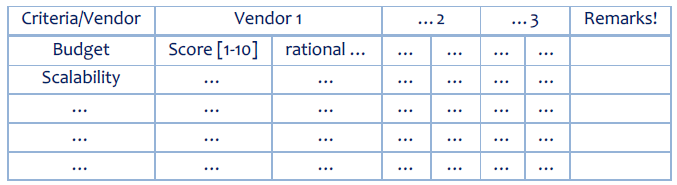
\includegraphics[width=0.5\textwidth]{Figures/Q7_QUESTION_table.PNG}
    \label{fig:my_image}
\end{figure}

\emph{[00:15:13] question number seven that's a web exercise and and i have talked about that
um in the beginning of the lectures so i recommend a data warehouse engine so a dbms engine for the
census office of course if you google you will um the term i mean what is the data warehouse engine used
for example by the swedish census office or finnish or us or german or etc they all are using by the way
and then you will get some uh case studies telling yeah those are using for example oracle technology
those are using pulse to grass and those are using teradata and yeah uh green plum and a lot of names
it's only uh some names that i have put here so so that the question here that i want to
yeah uh like test your ability to compare and recommend the technology so the name is not important so for
once again there is no model answer here to the name so for example if you ended up saying it's a tie db
and somebody else said no it's a single store and third student said it's a click house you all might
be right yeah as long as you have evaluated those options and put a criteria this is an exercise on
evaluation rather than an exercise on selection uh can we evaluate yeah what are the evaluation criteria
i put examples here like scalability and i talked about scalability in the course
or budget which one is cheaper uh yeah or which one is most expensive usually the cheapest gets the
highest points and the most expensive gets the lowest points when it comes to the budget criteria
which one is a scalable horizontal and vertical and we have talked about this and so forth so so you need
to collect the data um and compare}\\

What to do here?
\begin{enumerate}
    \item Choose three vendors
    \item Choose 5 criteria
    \item Evaluate each vendor in each criteria (in a table, see question)
    \item Summarize and recommend a DW DBMS for Census Bureau
  \end{enumerate}
\newpage Answers to Question 7:
testref \cite{benchmark}
\section{The Web Exercise}
This question requires a web exercise,therefore we have decided to add sections, one for each product. 

\subsection{Choice of criteria:}
The criteria we have chosen to evaluate the vendors and why are:
\begin{itemize}
    \item Scalability: This is an important criteria since:
    \begin{quotation}
        "Can we scale up, so this is important [...] the goverment is opening up it's database to the public for example.[...] so scalable means it can support more users and larger data volume"\cite[t.00:53:00]{l1video}".
    \end{quotation}
    \item Storage: Storage is an important criteria since
    the DBMS must efficiently handle large volumes of data, 
    ensuring optimal load performance and storage management to 
    accommodate growing datasets without architectural limitations \cite[p. 1239]{CourseLitt}.
    \item Cost: This is an important criteria since developing a DBMS is a costly endeavour, and the cost of the chosen DBMS can add or substract from this. \begin{quotation}
        "the cost can vary enormously from tens of thousands to millions of dollars due to
    the variety of technical solutions available." \cite[p. 1226]{CourseLitt}
    \end{quotation}
    \item Security: \begin{quote}
        "Security is critical to the data warehouse. To provide the strongest possible
security and to minimize administrative overhead, all security policies are enforced
within the data warehouse."\cite[p. 1309]{CourseLitt}
    \end{quote}
    \item Latency: This is an important criteria since \begin{quotation}
         "the DBMS must be able to handle large, complex queries for key business operations that must complete in reasonable time periods." \cite[p. 1239]{CourseLitt}
    \end{quotation} 
\end{itemize}
\subsection{Vendor 1 - ClickHouse:}
    
\subsection{Vendor 2 - SingleStore:}
    
\subsection{Vendor 3 - PostgreSQL:}

\section{The Comparison}
In this section we provide a comparison between vendors, therefore we have decided to add sections, one for each criterion. 

\subsection{Criteria 1 - Scalability:}
 
\subsection{Criteria 2 - Storage:}

\subsection{Criteria 3 - Cost:}

\subsection{Criteria 4 - Security:}

\subsection{Criteria 5 - Latency:}


\chapter{Question Eight}
The big challenges we see in implementing AI in a conventional BI architecture as shown in this course is that AI needs massive amount of data, 
and it ought to be unstructured data \cite{IBM_Structured_vs_Unstructured_Data}.
The conventional BI architecture as shown in this report is designed to handle unstructured data at such a scale \cite{Data_Lakes_Article}.
A way we would solve this would by not using an integrated ETL process, but rather an ELT process, where we extract data from external and internal sources,
load the data into a data lake, and then transform it from the data lake \cite{ETL_vs_ELT} into our current architecture (see Chapter 1\ref{sec:question1}).
This would allow us to store all the data in its raw form, and then use it to train models for AI upon the data-lake.
As such, we would need to add a data lake to the architecture, and connect the sandbox to the data lake to test models and 
algorithms before they are put into production.

We would also recommend employing an OLAP tool with good support for AI integration, 
and use vector databases to store data as to optimize it for AI usability \cite{Oracle_Vector_Database}.
As vector databases can be of a columnar storage structure type \cite{Oracle_Vector_Database}, the data in the BI-architecture would still be optimized for 
storing and querying large amounts of data,
with the expanded benefit of being optimized to store data for AI and AI-enhanced analytics needs.

A data lake is as the name suggest a big pool of unstructured data, and as such,
 data privacy and security should be a top priority when implementing this \cite{AWS_Securing_Protecting_Managing_Data}. 

So in summary, our changes to the architectureq would be to add a data lake, extract and load into that data lake, 
and then transform data from there into our current architecture.
We would also connect the sandbox to the data lake, employ an OLAP tool with good support for AI integration and 
use vector databases of the columnar data type to store data and 
increase security measures to mitigate some security risk from storing large and raw data in a datalake.



\chapter{Question Nine}
Question:\\
\begin{em}
Field exercise:

\begin{itemize}
    \item Contact either a Census Office, a Data Warehouse vendor, or a Data Warehouse
    Customer \{could be a government agency or private business\}.
    
    \item The contact could be anywhere geographically, preferably in Sweden/Nordic
    country.
    
    \item The person should have experience with the data warehouse, e.g., data
    warehouse consultant, ETL consultant, DW administrator, DW designer, DW presales
    engineer, Business/Data Analyst, Data Scientist, or a Manager using the
    data warehouse.
    
    \item Ask the person you will contact five questions:
    \begin{itemize}
        \item What is the value of a data warehouse in decision-making?
        \item Which decisions could be supported via the data warehouse?
        \item What is the role of analytics sandboxes in today's business intelligence environment?
        \item How to select an OLAP tool?
    \end{itemize}
    
    \item The answers to the above five questions could be obtained in a phone interview,
    via email, or face-to-face meeting.
    
    \item Report the organization's selection, the person, their answers, and your
    reflections on the answers you have obtained in your report.
\end{itemize}
\end{em}

\emph{[00:18:45] the last question is about the field exercise we learn things in that course and then
it would be great if we can also hear from experts or specialists consultants so so you need to contact
maybe the census office a data warehouse vendor like those names up here or otherwise microsoft oracle ibm etc any
one of those names including as well and then ask that could be a government also agency using
data warehousing data warehousing or a private sector and it's almost everybody is doing so and then ask
preferably in sweden but it's also okay to have that person from outside the nordics ask different
questions yeah but the person should have expertise with data warehousing or etl or data warehouse
administration data warehouse design uh like a sales engineer a consultant business analyst the data
scientist or a data warehouse manager so so this is like propose the titles for the persons that you could interview
interview and then ask them those questions what is the value of a data warehouse in decision making
which decisions could be supported via the data warehouse what is the role of analytic sandbox in
today's business intelligence environment and how do you select an olap tool then you need to report
the interview and the answers of that person you will interview to the questions and \textbf{then put your
insights has that brought new knowledge to you does this come in line with the knowledge that you have
obtained in the course or is it against what you have learned this has triggered some new knowledge to me
this has motivated me to do more research etc so i want you to add your reflection on the answers that
you have obtained yeah and then that all goes into a report}}\\

What to do here?
\begin{enumerate}
    \item 
  \end{enumerate}


\newpage Answers to Question 9:
\section{Person}
Due to confidentiality agreement with the company, the person's name and the company's name cannot be disclosed. The person is thus described as:
Anonymous data engineer (primarily working in the ETL layer). The interviewee disclosed that their educational background is a master degree in computer science.

\section{Organization}
This section profiles the organization at which the person with whom we have conducted the interview is working. 
Due to confidentiality agreement with the company, the company's name cannot be disclosed. The company is thus described as:
A big international Swedish housing development company with around 1000 employees.
\section{Interview Questions}
Here is the summarized answers for the interview followed by a subchapter about our reflections on those answers. See Appendix~\ref{sec:interview} for the full transcript.
\subsection{Question 1: What is the value of data warehouse to decision making?}

In the interview a representative from a housing development company emphasized the critical role of their data platform 
in decision-making. While they use a data lakehouse rather than a traditional data warehouse, the platform provides valuable 
insights across multiple areas, including finance, health and safety, sales, and marketing.

For example, project leads access continuously updated reports to monitor cost trends, safety compliance, and project performance. 
This enables them to quickly identify cost overruns and optimize spending. Marketing teams use the platform to track campaign 
effectiveness, assessing ROI across different channels to refine their strategies. Similarly, sales teams analyze data to understand 
which projects sell quickly and which require additional effort, helping optimize pricing and marketing tactics.

Overall, the company's centralized data platform enhances operational efficiency, financial oversight, and strategic planning, 
demonstrating the importance of robust data infrastructure in modern business decision-making.
\subsubsection{Reflections on answer to question 1}
A Data Lakehouse (DLH) was mentioned in the interview, a hybrid type of warehouse that combines the benefits of both Data Lakes and Data Warehouses. 
Unlike traditional Data Warehouses (DWH), which focus on structured data, DLHs allow for a mix of structured and unstructured data, 
providing greater flexibility and real-time analytics \cite{datalakehouse}. This is especially useful for continuous decision-making, like in the housing company example. 
It would be beneficial to explore the differences between DWH and DLH further, as their differences weren't covered in the course.

The company's platform offers insights across various business areas, similar to how Data Warehouses provide insights across multiple domains in the course material. 
The platform supports decision-making in finance, health and safety, and marketing, highlighting the importance of having centralized, up-to-date data for strategic decisions. 
This aligns with the role of DWHs in consolidating data for business intelligence.

\subsection{Question 2: Which decisions you think could be supported via the data warehouse?}

In the interview it was explained how the company's data lakehouse plays a key role in decision-making. While primarily relying on 
internal data, they are actively exploring ways to integrate external market trends to enhance their analytical capabilities.

The platform allows project leads to monitor costs in real time, helping them identify overruns and adjust spending accordingly. 
Marketing teams use data insights to assess campaign performance and optimize ad placements on platforms like Google and YouTube. 
Sales teams analyze trends to determine where additional marketing efforts are needed and whether pricing strategies should be adjusted. 
Additionally, by reviewing past project success, the company refines its future investment and development strategies.

Looking ahead, they aim to incorporate broader housing market data and industry trends, which would provide a more comprehensive basis 
for strategic decision-making.
\subsubsection{Reflections on answer to question 2}

The integration of external data with internal data is mentioned as providing a richer and more holistic view, enhancing decision-making processes. 
It would be valuable to explore how such integration is implemented in data warehouses (DWH), as this could offer a deeper understanding 
of how to analyze external market trends which shape business strategies. Further investigation into the different sources and types of external data 
would be an interesting area for future study, especially in the context of DWH and business intelligence.

Real-time monitoring is a crucial feature in DWH systems \cite[p. 1230]{CourseLitt}. Observing how it is applied in practice, such as tracking project costs, 
could offer a practical example of its impact on decision-making.

The use of external data to predict future trends is a compelling aspect. By incorporating external market trends, the company can potentially 
anticipate shifts in the housing market and adjust its strategies accordingly. A deeper analysis of how external data sources contribute to forecasting 
and trend analysis would be useful for understanding its role in strategic decision-making. This could open avenues for more proactive planning, 
especially in volatile or dynamic markets.

\subsection{Question 3: What is the role of analytics sandboxes in today's business intelligence environment?} 

The representative discussed how they do not use a traditional analytics sandbox, but instead operate with flexible environments that 
serve similar functions. Their system is built on a data lakehouse, and they maintain development, test, and production environments 
to support rapid development and experimentation. These environments allow teams to test new hypotheses and analysis methods without 
affecting the production environment.

The company also uses Apache Spark and Parquet files, which enable them to conduct ad hoc analysis in a flexible, low-risk way. The 
use of Jupyter Notebooks provides the ability to test and visualize data quickly, making it possible to try out different approaches and 
gather insights without disrupting ongoing operations. This setup supports rapid development cycles and allows for fearless experimentation 
in a way that is similar to the benefits provided by an analytics sandbox.
\subsubsection{Reflections on answer to question 3}

The DLH approach offers more flexibility for experimentation compared to traditional DWH, which often limits rapid iteration \cite{datalakehouse}. 
It's interesting how DLH integrates structured and unstructured data for dynamic development cycles. It could be of interest
to learn more about the similaities and key differences between DLH and sandboxes in DWH in relation to analytics.

The use of Apache Spark and Parquet files for ad hoc analysis is intriguing. It would be beneficial to explore how these tools compare to
traditional BI tools in terms of flexibility and user experience would be beneficial. This comparison could provide insights into the advantages and limitations of each approach, helping to determine the most suitable tools for various analytical needs.
The use of Parquet files for storage means they are using a columnar storage format, which is known for its efficiency in handling large datasets \cite{apache_parquet}.
the use of Apache Spark seems to be a popular, scalable engine for big data processing with machine learning tool support \cite{apache_spark}, it would be interesting to learn more of it's core role in the Data LakeHouse environment in comparrison to the different parts of a Data Warehouse.

\subsection{Question 4: How to select an OLAP tool?}

The representative explained that their company does not use an stricly speaking OLAP tool within their data team, but instead uses a tool called Power Bi which they find sufficient for their analytical needs. 
Another team, the statistics team, does however use an OLAP tool, which name cannot be disclosed due to confidentiality agreement. 
When selecting an OLAP tool, performance is a key consideration, particularly the ability to store all data in memory rather than on disk, which 
provides significant performance benefits. However, this approach can lead to high costs due to the high and expensive memory usage.

The company is currently exploring alternatives to their existing OLAP tool, considering non-OLAP tools like Spark and Power BI for certain use cases. 
The representative noted that for their team, Spark and notebooks already fulfill many of the functionalities required for ad hoc analysis, 
offering a more flexible and cost-effective solution compared to their current traditional OLAP tool.

\subsubsection{Reflections on answer to question 4}

The use of Power BI instead of traditional OLAP tools is an interesting shift, as it highlights a more flexible and cost-effective approach
in comparison to their current OLAP tool. 
However, this raises the question of when OLAP tools become essential. They seem to be needed when the complexity of analysis or the volume 
of data requires fast, multidimensional querying \cite[p.1288]{CourseLitt} that tools like Power BI may struggle to handle.

The trade-off between performance and cost is a key insight. In-memory storage can deliver impressive performance but at a high price. 
While OLAP tools may be ideal for speed and complexity, alternatives like Spark and Power BI seem to offer a more balanced approach,
in the interviewee's organisation, 
especially when cost efficiency becomes a priority. 
It makes you think about how organizations really have to weigh the value of performance against financial limitations and 
to perhaps be restricive in their approach to when and how to implement in-memory based OLAP tools.







\chapter{Conclusion}
In this report, we have thoroughly examined various aspects of database management systems (DBMS) 
and their applicability to a Census Bureau's needs. 
We viewed the different compontent of a BI-architecture and their applicability for a Census Bureau.

% BI-architecture elements
We concluded that data marts and sandboxes are an important part of a BI architecture,
as they provide a structured environment for data analysis and experimentation while still being restrictive and carefull in their implementation.
Data mining was concluded to be a crucial part of a BI architecture,
as it enables the discovery of patterns and trends in large datasets.

%analysis of each DBMS
Through a detailed comparison of ClickHouse, SingleStore, and PostgreSQL, 
we have evaluated their performance based on criteria such as scalability, 
storage, cost, security, and latency.
Our analysis revealed that each DBMS has its strengths and weaknesses. 
ClickHouse emerged as the best overall choice due to its superior performance in 
security and latency, which are critical for a Census Bureau. 
Its open-source nature and cost-effectiveness further enhance its appeal. 
SingleStore, while excelling in scalability and storage, 
falls short in terms of cost and security compared to ClickHouse. 
PostgreSQL, despite being a robust and reliable DBMS, lags behind in several key areas, 
making it the least recommended option for this specific use case.



% AI integration
We also explored the challenges and solutions for integrating AI into 
a conventional BI architecture. 
By proposing the addition of a data lake and the use of ELT processes, 
we addressed the need for handling large volumes of unstructured data. 
The integration of vector databases and enhanced security measures further ensures that 
the architecture is optimized for AI-enhanced analytics.

% interview
From the interview discovered the concept of Data Lake House (DLH) and tools used in its implementation,
in the future it would be interesting to explore in greater detail the possibility of implementing a DLH in a Census Bureau.

In conclusion, the best DBMS for a Census Bureau, 
considering the importance of security, latency, and cost, is ClickHouse. 
However, it is essential to adopt a balanced approach, 
leveraging the strengths of each DBMS where applicable, 
to build a robust and efficient data management system. 
The proposed architectural changes will enable the Census Bureau to harness the power of AI, 
ensuring that it remains at the forefront of data-driven decision-making.
Dwelving deeper into the subjects uncovered in the interview before doing so could 
however greatly change the design of the warehouse. 


\chapter{Appendix}
\section{Interview Transcript} \label{sec:interview}
\begin{quote}
    \textbf{Interviewer:} What is the value of data warehouse decision-making in your organization?
    
    \textbf{Interviewee:} well at our place we use um our we don't strictly use the data warehouse but rather data lakehouse and our data platform provides quite a lot of value when it comes to decision making.

    We use it for things like finance, health and safety, sales, marketing and yeah a bunch of other different places... It's a little bit case by case basis but you know we're
    a housing development company so one instance would be that the project leads for any of our housing projects they have a continuously updated report where they can track the economics and the health and safety and all of the things that they need to be on top of to see how things are developing with their projects
    
    And this kind of enables them to see the data see trends, if we're having cost overruns what part of the construction project is it happening in and is there any way to
    you know make this cost go away. That's one case. 
    Same thing with our marketing people they use this to track where they spend the money, what are the returns on investment by marketing different channels, this helps them to evaluate each campaign they drive through, and at the end of the day they can look at what what did they put in what did they get out and they can decide if they want to move to making the next smart campaigns in other areas or if they'd rather continue more in the same area.
    
    Or for instance if you want to do your ads on Google or Youtube.
    
    Same thing with sales our whole sales pipeline is very connected to... we have a CRM system of course like everyone else does but everything is aggregated connected to and aggregated to our data platform or rather connected to and aggregated within our data platform.
    
    So we can look at more of the overarching trends for sales and see what projects are we building where sales are going slow where are they going quickly.
    And these things are great both to see what projects we have which would need more love in the sales and where we could put more effort into getting these units sold, because having an empty apartment for any stretch of time is a waste of money.
    But in the same way this can also be used retroactively at the larger scale to look at what type of projects has turned out to be very lucrative and also what has turned out to be very hot on the market and make evaluations on maybe we're underpricing things if we sell at a very high pace, or maybe we're overpricing things if we sell things at a too slow pace.
    
    Same thing. I don't know. You want me to keep coming up with examples or...

    \textbf{Interviewer:} No thank you, that should be sufficient.

    \textbf{Interviewee:} Good to hear.

    \textbf{Interviewer:} Next question then, Which decisions could be supported via the data warehouse?

    \textbf{Interviewee:} Well, so as I mentioned before, we are already using it for decision support to quite an extent. But we're mostly working with our own data. And one of the directions we've started looking at and trying to figure out is how can we incorporate more external data than we are today, and look at things like, how is the housing market doing in general? What are current trends on you know, with construction work and housing development? What kind of trends are we seeing in general with marketing? And just this kind of work with incorporating data from a much broader range of sources, and trying to incorporate those in our analysis, those, I think would be something which we could support, which we don't do as of yet.

    \textbf{Interviewer:} Great, thank you. And machine learning, what do you think could be useful there?

    \textbf{Interviewee:} Yeah, I think that's a very good question.I think we could use machine learning for a couple of different use cases. One which is very strong, but maybe a bit boring is automation and efficiency. Because we just as every organization, or every person on this planet, we have a bunch of repetitive tasks. And we can use machine learning to automate them. We already do this for automate automatic categorization of invoices to help out the finance department. And this has been very useful to have the data underlying this, of course. But then I think we could also start looking at machine learning models or other types of advanced analytics to spot patterns in the market and figure out what kind of decisions we should make. And if there's any good predictors for what is going to be a lucrative project or not for us.

    \textbf{Interviewer:} *And that's where the external data sources come in as well, I guess.

    \textbf{Interviewee:} Yeah, exactly. Yeah, for machine learning. That's what we'd use the combination of our own and external data, of course.

    \textbf{Interviewer:} Okay, thank you. Next question then. What is the role of analytics sandboxes in today's business intelligence environment?

    \textbf{Interviewee:} Well, so I'm speaking in a bit of an odd position here, because we don't strictly speaking, have an analytic sandbox.

    We at because we work with a quite flexible system from the get go, as opposed to data warehouse we work with a data lakehouse.
    
    And we also all of our code is in Spark, and all of our data is stored in (Apache) Parquet files.
    
    So, but with that said, we do have a development test and production environment more like software developers would do it. 
    And with this we have a development environment where we can do... either we can create artificial or hypothetical data to try out some kind of hypothesis with our current analysis versions, or we can look at current like real current data and try new analysis methods, or we can do any combination of them.
    And we're connected to all the different data sources in their environments as well so we can take in hypothetical data which is created in other systems so we have a lot of flexibilities in the ways we work which I think is what you want to get out of an analytic sandbox.
    
    And this is great for us because we can both... we can very quickly develop and we can try out new features at a high pace without having to modify our production environment and we can actually be very fearless in our work and we can move rapidly and this is one of the main points for us at least and i think for anyone using an analytic sandbox.
    Other than that we do have like the tool we work with for all of our calculations and transformations generally is Spark.
    
    And one of the main perks with Spark is that it's very very flexible in how you want to work with it. 
    For example, all of our automatically running transformations in pipelines we work with with Spark jobs which is more like a script and they're very rigid we you know we develop them we move them through our different environments we test them we publish them.
    But on the other hand you can just as well use Spark with something called the Notebook and that is very much made for an *ad hoc* analysis so you get great performance because Spark is distributed but you can very very rapidly work your way through problems and you have a very good integration between writing code but also visualizing it in a super helpful way so that's that's probably the most sandboxy thing we do.

    \textbf{Interviewer:} *Okay, great. Thank you. So, to understand it a bit, what you're trying to say, in part at least, is that analytical sandboxes can help a lot with what's called ad hoc questions and such things?

    \textbf{Interviewee:} yeah I'd say they're good both for trying out things and developing things which are gonna at some point be less of an *ad hoc* situation, just as well, every now and then the business needs some kind of quick analysis for something super specific where we're gonna do this one time and then doing this kind of analytic sandbox solution where you can just throw it out there see the numbers and see what they return that is super helpful as well definitely.

    \textbf{Interviewer:} Thank you. Last question then, how to select an OLAP tool?

    \textbf{Interviewee:} Yes, very good question. So at our company my team which is the data team we don't really work with an OLAP tool we do have a different team who does work with the OLAP tool i think would be a multi-dimensional one and i think they've selected it on a number of different things.

    One of the main things I know when they got it was performance. It loads the entire data, all the data that it works with, is stored in memory instead of on disk which obviously gives you very good performance benefits, and it's great for looking at high dimensionality data. 
    But i know they've had some issues with the costs getting away quite quickly because everything is in the memory and not on disk...
    
    And another part which I think if I was in charge of selecting an OLAP tool I'd probably look a lot at the kind of development operations regarding it and see that you can work with it in more of the software development ways where you do agile development you have **CI/CD** (continuous integration/continuous delivery) you work with version control because these things have been a challenge from the get-go for them.
    
    But my team on the other hand we do some of the same things you would do in an OLAP tool and yeah maybe I should mention that at there is currently an ongoing investigation going for phasing out the OLAP tool we currently use at my company.

    \textbf{Interviewer:} the MOLAP tool?

    \textbf{Interviewee:} yeah the multi yeah exactly.

    What we do instead is i think for some of the use cases where you use an OLAP tool of the Spark and notebooks for that kind of quick analysis, moving through the data, trying to figure it out, seeing how it works.
    That on one hand is solved there mostly for us.
    And then on the other hand, the kind of ease of use, nice visualizations, being able to as a kind of end user or a business user for us, they can go through our data and look at it through something like Power BI, which is, it's mostly two dimensional flat, but it's very good given that we, you know, help them, we make nice data sets where everything is reasonably structured.
    You can move through the data and look, you can go up and drill up, drill down, you can do slicing and you can do all of these things to explore the data in there in an easy to use fashion, while not going the full extent, not having something as heavy as an OLAP tool, maybe.

    \textbf{Interviewer:} okay, so it's almost an OLAP cube but not fully...?

    \textbf{Interviewee:} Yeah, I think, I think we have, let's call it a OLAP square in Power BI.
    At least that's the way we use it.
    It could possibly be that you can represent data in more higher dimensionality, but the way we work with it is with two dimensional data.

    \textbf{Interviewer:}So what do you use Power BI for since that's like your pseudo-OLAP tool if I understand that correctly? It's like what you use instead of an OLAP tool so to say.

    \textbf{Interviewee:} So we use it kind of on two ends of the spectrum.
    We have some reports, which we ourselves, we design them and we make them kind of as a ready to use pre-configured, all the metrics are there, all the charts are there. 
    And then the end users, which, you know, might be anyone in the marketing or health and safety or finance department, they get just a continuously updated report where they can navigate around and do some, they can work, they can, you know, they can still drill up, drill down and slice stuff, but it's quite predefined.
    But on the other hand, more within the team and for some of the more power users, we use it so they can pull in slightly rawer data and they can structure it and go through it and kind of explore; data exploration I would probably say it would be the more internal use for the more power users, but while still being a no code environment where you can do kind of drag and drop analysis, I guess you could call it.

    \textbf{Interviewer:}Okay, so when it comes to how to select an OLAP tool in your organization it seems like if there's somewhat of a focus on it being easy to interact with without there being too much of a technolgical barrier?

    \textbf{Interviewee:}Yeah, it should be without too big of a technological barrier.
    It should be, we try to make it so that we do the more heavy lifting and all those things are on the data engineering side and in the data lake house with Spark.
    And then we produce nice data which can be interacted with in a friendly user interface through something like Power BI.
    And I think for us, it works very well.
    But that, again, has a lot to do with us doing a lot of the heavy lifting before getting the data into Power BI
    and having really nice data, which is all quite often,
    we already aggregate some of the data that needs aggregation.
    We filter out all of the data, which definitely should not go in there.

    \textbf{Interviewer:}And you think the tools in Power Bi are sufficient for your use-case or do you think it is lacking in some way?

    \textbf{Interviewee:}I think for us, it works very well. But that again has to do with us doing a lot of the heavy lifting before getting the data into Power Bi. And having really nice data which is quite often already aggregated and filtered. So for our use case, I think it's perfect.
    But if you worked somewhere where you had a data platform which couldn't do as much of the heavy lifting and was more of a just storage place for your data,
    then I think you would need to have something a bit more powerful than, say, Power BI, because it gets bogged down once you get to, it doesn't have the performance of, for instance, our old OLAP tool where you can just put in very large amounts of data and peruse through it anyway you want.
    If you want something like Power BI, you have to be a little bit more careful, I'd say.
    But for us, perfect.

    \textbf{Interviewer:}*Okay, okay, and do you know what OLAP tool you're using or you can't say perhaps?

    \textbf{Interviewee:} I am not sure I can say.

    \textbf{Interviewer:} Okay, well, that's okay, that's okay, that's fine.

    \textbf{Interviewee:} But it's one of the big ones.

    \textbf{Interviewer:} Okay, yeah, that's great. Okay, well, thank you very much. That's all the questions. Thank you for taking part in the interview.

    \textbf{Interviewee:} Again, no worries.

\end{quote}

\printbibliography

\end{document}